\chapter*{Introduction}

Pour ce projet, le sujet abordant le système de particules (numéro 2) a été
retenu. Le choix de ce sujet s'est fait sur l'intérêt de la gestion physique de
ces particules de manière efficace. Dans les jeux vidéos, les systèmes de
particules sont trop peu souvent utilisés, pour gérer des phénomènes tels que la
fumée ou le feu, au profit de simples sprites (ce phénomène est toujours présent
même dans des jeux récents, à l'instar de Watch\_Dog).\\

\begin{center}
	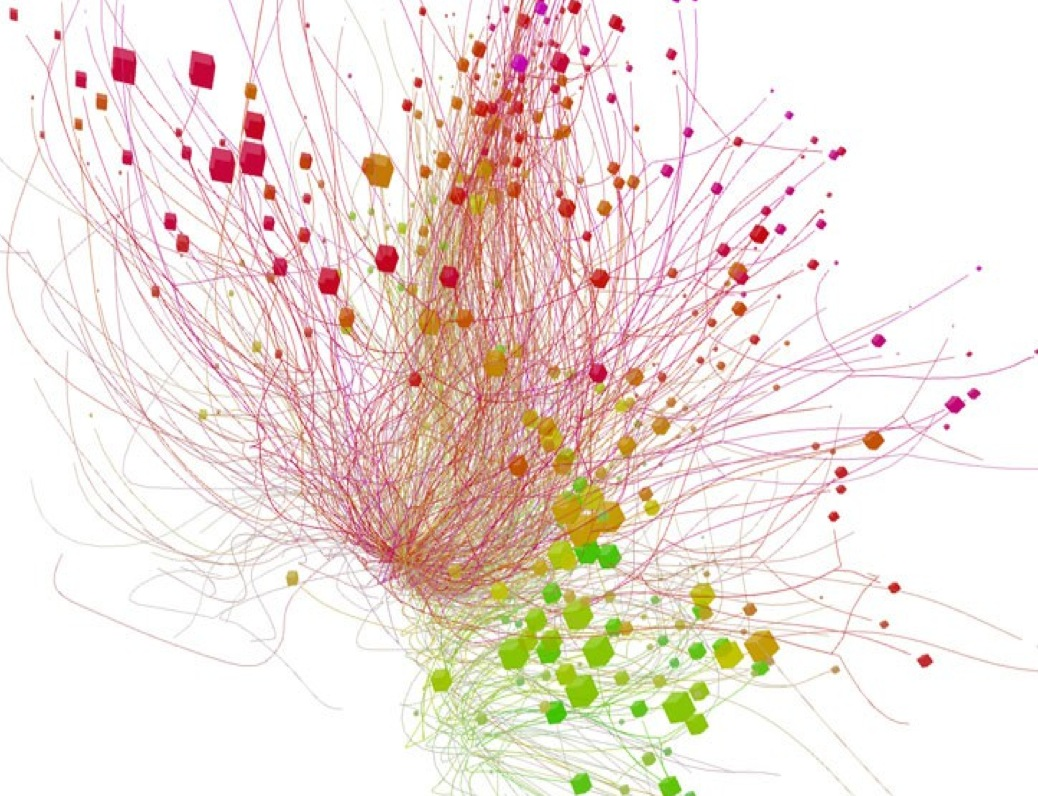
\includegraphics[width=0.7\textwidth]{img/01-introduction.jpg} 
\end{center}

Dans une première partie, le projet ainsi que les objectifs fixés seront
présentés. Les différentes phases de réalisation et d'implémentations de
l'application seront ensuite abordés. Ce rapport se terminera sur l'évocation
des problèmes rencontrés tout au long du projet, et les possibles améliorations
à apporter.
